\documentclass[10pt]{article}
\usepackage{geometry}
 \geometry{a4paper}
\usepackage{fancyhdr} % Required for custom headers
\usepackage{lastpage} % Required to determine the last page for the footer
\usepackage{extramarks} % Required for headers and footers
\usepackage[usenames,dvipsnames]{color} % Required for custom colors
\usepackage{graphicx} % Required to insert images
\usepackage{listings} % Required for insertion of code
\usepackage{courier} % Required for the courier font
\usepackage{lipsum} % Used for inserting dummy 'Lorem ipsum' text into the template
\usepackage{caption}
\usepackage{subcaption}
\usepackage{amsmath}
\usepackage{amsmath}
\usepackage{amssymb}
\usepackage{epstopdf}
\usepackage{placeins}
\usepackage{color} 
\usepackage{fancyvrb} 
\usepackage{setspace}
\usepackage[numbered]{bookmark}
\usepackage{pdfpages}
\usepackage{enumitem}
\usepackage{tikz}
\usepackage{pgfplots}
\DeclareGraphicsExtensions{.pdf,.png,.jpg}
\graphicspath{{../figs/}}

\usepgfplotslibrary{fillbetween}
\usetikzlibrary{positioning}

\usetikzlibrary{pgfplots.groupplots}
\usetikzlibrary{plotmarks}
\usetikzlibrary{calc}

\usepgfplotslibrary{groupplots}

\pgfplotsset{compat=newest} 

\DeclareMathOperator{\E}{\mathbb{E}}

\begin{document}
\doublespacing
\section*{Nonlinear Plant Identification}

\subsection*{General description}

As discussed in class, we can use adaptive filters to model unknown plants. In many practical applications, however, the plant may exhibit some nonlinear characteristic that cannot be accurately modeled by linear filters. In this exam, you'll design and compare linear and nonlinear adaptive filters to model a given nonlinear plant.

The typical block diagram of plant identification problems is shown in Figure~\ref{fig:block-diagram}. An input signal $r_k$ is presented to the plant and to the adaptive filter. The output of the plant $d_k$ is the desired response that we use to compute the error $\epsilon_k$. As usual, the output of the adaptive filter $y_k$ is expressed as the inner product of an input vector $X_k$ and the weight vector $W_k$. In a linear adaptive filter, the input vector depends only on linear or affine terms of the input $r_k$, whereas in a nonlinear adaptive filter, the input vector also contains some nonlinear terms of the input $r_k$.

\begin{figure}[h!]
	\flushleft
	\resizebox{\linewidth}{!}{\def\layersep{1.5cm}
\def\outsep{0.7cm}
\def\dy{1.25}

\begin{tikzpicture}[->, >=stealth, shorten >= 0pt, draw=black!50, node distance=\layersep, font=\sffamily]
\tikzstyle{node}=[circle,fill=black,minimum size=2pt,inner sep=0pt]
\tikzstyle{weight}=[draw=black,circle,fill=none,minimum size=3pt,inner sep=0pt,font=\fontsize{6}{6}\selectfont]
\tikzstyle{summer}=[weight, minimum size=15pt, inner sep=2pt]
\tikzstyle{block}=[draw=black,rectangle,fill=none,minimum size=1cm, inner sep=0pt]
\tikzstyle{annot} = []

\node[node] (rk) at (0, -\dy cm) {};
\node[node] (in) at (0.25*\layersep, -\dy cm) {};
\node[block] (H1) at (1*\layersep, -\dy cm) {$H_1(z)$};
\node[block] (g) at (2*\layersep, -\dy cm) {$g(\cdot)$};
\node[block] (H2) at (3*\layersep, -\dy cm) {$H_2(z)$};
\draw[-, dashed] (1*\layersep-0.75cm,-\dy*0.5) rectangle (3*\layersep+0.75cm,-1.5*\dy);
\node[annot, below=4pt] at (2*\layersep, -1.5*\dy) {``Unknown'' plant};
\node[node] (plant-out) at (4*\layersep, -\dy cm) {};
\coordinate (output) at (4.5*\layersep, -\dy cm) {};
\node[summer] (error) at (4*\layersep, -2*\dy cm) {\Large $\Sigma$};
\coordinate (error-out) at (4.5*\layersep, -2*\dy cm) {};

\draw (error-out) -- (4.5*\layersep, -3.75*\dy cm) -- (2.5*\layersep, -3.75*\dy cm) -- (1.5*\layersep, -2.3*\dy cm);
\node[block, fill=white, minimum width=3cm] (adapt) at (2*\layersep, -3*\dy cm) {Adaptive filter};

\path[-] (rk) edge (in);
\path (in) edge (H1);
\path (H1) edge (g);
\path (g) edge (H2);
\path[-] (H2) edge (plant-out);
\draw (in) |- (adapt);
\draw (plant-out) -- (output);
\draw (plant-out) -- (error);
\draw[-] (error) -- (error-out);
\draw (adapt) -| (error);

\node[above right = 0.5mm and 0.1mm of error, scale=0.8] {$+$};
\node[below right = 0.5mm and 0.1mm of error, scale=0.8] {$-$};
\node[left = -2mm of rk, text width = 2cm, align=center, scale=0.8] {Plant input \\ $r[n]$};
\node[right = -2mm of output, text width = 3cm, align=center, scale=0.8] {Desired response \\ $d[n]$};
\node[scale=0.8, below right = -5mm and 1mm of adapt] {$y[n] = X_n^TW$};
\node[right = 1mm of error-out, align=center, scale=0.8] {error \\ $e[n]$};



% 	\node[summer] (Adder) at (3*\layersep,-\dy*2.5 cm) {\large $\Sigma$}; 
%     \node[node, inner sep=0pt] (mid) at (4.5*\layersep,-\dy*2.5 cm) {}; 

%     \node[node, inner sep=0pt] (output-tap) at (7.3*\layersep,-\dy*2.5 cm) {};
%     \coordinate (output) at (8*\layersep,-\dy*2.5 cm) {};
%     \node[summer, minimum size=10pt] (error) at (6*\layersep,-\dy*5 cm) {$\Sigma$}; 
%     \coordinate (xw) at (4.5*\layersep,-\dy*5 cm) {};
%     \coordinate (out) at (7.3*\layersep,-\dy*5 cm) {};
%     \node[weight,fill=white] (gamma) at (4.5*\layersep,-\dy*4 cm) {\small $\gamma$};
%     \coordinate (error-out) at (6*\layersep,-\dy*6 cm) {};


%     \coordinate (A) at (\layersep,-6*\dy cm) {};
%     \coordinate (B) at (\layersep,\dy cm) {};
%     \path (A) edge (B);
%     \path[-] (error) edge (error-out);
%     \path[-] (error-out) edge (A);

%     \foreach \name / \y in {0,...,3} {
%     % This is the same as writing \foreach \name / \y in {1/1,2/2,3/3,4/4}
%         \node[node] (I-\name) at (0,-\dy*\y) {}; % Draw the input layer nodes
%         \node[weight,fill=white] (W-\name) at (\layersep,-\dy*\y cm) {$W_\name$}; % Draw the hidden layer  layer node     
%      }   	

% 	\node[node] (I-4) at (0,-5*\dy cm) {}; % Draw the hidden layer 
% 	\node[weight, fill=white] (W-4) at (\layersep,-5*\dy cm) {$W_n$};

%     %% Annotations
%     \node[annot] at (-0.3,0) {$+1$};
%     \node[annot] at (-0.3,-\dy) {$X_{k1}$};
%     \node[annot] at (-0.3,-\dy*2) {$X_{k2}$};
%     \node[annot] at (-0.3,-\dy*3) {$X_{k3}$};
%     \node[annot] at (-0.3,-\dy*5) {$X_{kn}$};
%     \node[annot] at (-0.3,-\dy*3.75) {$\vdots$};

%     \node[font=\fontsize{3}{3}\selectfont] at (6*\layersep-7,-\dy*4.7 cm) {$-$};
%     \node[font=\fontsize{3}{3}\selectfont] at (6*\layersep+7,-\dy*4.7 cm) {$+$};
%     \node[annot] at (3*\layersep+7,-\dy*5.7 cm) {$\epsilon_k$};
%     \node[annot, right of=output] {Output};
%     \node[annot, below of=SGM] {Sigmoid};

%     \foreach \name in {0,...,4} {
%     		\path (I-\name) edge (W-\name);
%             \path (W-\name) edge (Adder);
%      }

%     \path[-] (Adder) edge (mid);
%     \path (mid) edge (SGM);
%     \path[-] (mid) edge (gamma);
%     \path[-] (gamma) edge (xw);
%     \path (xw) edge (error);
%     \path[-] (SGM) edge (output-tap);
%     \path (output-tap) edge (output);
%     \path[-] (output-tap) edge (out);
%     \path (out) edge (error);


%% Text
%     \node[annot,left of=I1-3, node distance=1cm] (in) {\normalsize Inputs};
%     \node[annot,right of=O4-3, node distance=0.5cm] (out) {\normalsize Outputs};
%    \draw[decoration={brace,mirror,raise=5pt},decorate, thick, text width=3em, text centered]
%    (7.5, -4) -- node[below=6pt] {\normalsize LMS output layer} (8.5, -4);
\end{tikzpicture}}
	\caption{Block diagram for nonlinear plant identification problems. } \label{fig:block-diagram}
\end{figure}

Throughout this exam, we'll assume that the nonlinear plant has the structure shown in Figure 1. It has an input linear filter $H_1(z)$ followed by some nonlinear operation $g(\cdot)$, followed by another linear filter $H_2(z)$. We'll also assume that
\begin{equation}
H_1(z) = H_2(z) = -0.0078 + 0.0645z^{-1} +  0.4433z^{-2} + 0.4433z^{-3}+ 0.0645z^{-4} -0.0078z^{-5}
\end{equation}
\begin{equation}
g(u) = \exp(u/2) - 1.
\end{equation}

The nonlinear plant is provided to you in the Matlab function \texttt{nonlinear\_plant.m}. To calculate the plant output to an input signal \texttt{r}, you can simply call \texttt{d = nonlinear\_plant(r)}.

We'll consider two types of adaptive filters. In the first part of the exam, the adaptive filter consists of a finite impulse response (FIR) filter $F(z) = w_1 + w_2z^{-1}+\ldots+w_{L+1}z^{-L}$, and a bias weight $w_0$. Thus, we have a total of $L+2$ weights. A FIR filter is the typical transversal filter you have encountered many times in homework problems. The bias weight is simply a weight whose input is always $+1$. The bias weight is necessary because the plant nonlinearity $g(u)$ is not symmetric about $u = 0$. Therefore, the plant output may be biased even when the plant input signal has zero mean. The sole purpose of $w_0$ is to track the mean of the desired response $\E[d_k]$.

In the second part of the exam, the adaptive filter consists of a nonlinear filter based on the truncated discrete-time Volterra series\footnote{\normalsize You can think of Volterra series as a Taylor series with memory. In other words, the output depends not only on the input at present time $x(k)$, but it also depends on the input at past times $x(k-1), \ldots, x(k-L)$. The series used here is causal and it is truncated in time by $L$ past samples, and it is truncated on the number of cross products of the input $p = 1, 2$. Interestingly, it can be shown that Volterra series can model any dynamic nonlinear system with arbitrarily small error, provided that $L$ and $p$ are large enough.} shown below:
\begin{align} \nonumber \label{eq:volterra}
y(k) &= w_0 + \sum_{p = 1}^{2}\sum_{n_1 = 0}^L\sum_{n_2 = n_1}^L w_{p}(n_1, n_2)\prod_{j = p}^2x(k-n_j) \\
& = w_0 + \sum_{n = 0}^Lw_2(n)x(k-n) + \sum_{n = 0}^Lw_1(n)x^2(k-n) + \sum_{n_1 = 0}^{L-1}\sum_{n_2 = n_1+1}^L w_{1}(n_1, n_2)x(k-n_1)x(k-n_2),
\end{align}
where $x(k)$ is the input signal and $y(k)$ is the output signal.  $w_p(n_1, n_2)$ is commonly referred to as discrete-time Volterra kernel, but for our purposes, it will be weights of the adaptive filter. Note that we have abbreviated the notation by writing $w_1(n)$ and $w_2(n)$. Formally, $w_1(n) = w_1(n, n)$ and $w_2(n) = \sum_{n_1 = 0}^{n}w_2(n_1, n)$. Following this convention, $w_0, w_2(n), w_1(n)$, and $w_1(n_1, n_2)$ with $n_1\neq n_2$ are the weights of the adaptive nonlinear filter. 

As an example, Figure~\ref{fig:volterra-diagram} shows the block diagram of a nonlinear filter based on Volterra series for $L = 2$. Inspecting \eqref{eq:volterra} and Figure~\ref{fig:volterra-diagram}, we see that, as before, we have a bias weight $w_0$ and the weights $w_2(n), n = 0, \ldots, L$, corresponding to linear terms of the input $x(k),\ldots,x(k-L)$. But now we also have the weights $w_1(n), n = 0, \ldots, L$, which weigh the input squared $x^2(k),\ldots,x^2(k-L)$, and the weights $w_1(n_1, n_2), n_1\neq n_2$, which weigh the cross-products of the input at different times $x(k)x(k-1),\ldots,x(k-L+1)x(k-L)$. Thus, we have a total of $1 + (L+1) + (L+1) + \binom{L+1}{2}$ weights.

\begin{figure}[t!]
	\centering
	\resizebox{\linewidth}{!}{\def\layersep{1cm}
\def\outsep{0.7cm}
\def\dy{1.25}

\begin{tikzpicture}[shorten >= 0pt, draw=black!50, node distance=\layersep, font=\sffamily, cross/.style={path picture={ 
		\draw[black]
		(path picture bounding box.south east) -- (path picture bounding box.north west) (path picture bounding box.south west) -- (path picture bounding box.north east);
	}}]
\tikzstyle{node}=[circle,fill=black,minimum size=2pt,inner sep=0pt]
\tikzstyle{weight}=[draw=black,circle,fill=white,text width=0.9cm,inner sep=0pt, align=center, font=\fontsize{6}{6}\selectfont]
\tikzstyle{prod}=[draw=black,circle,cross,fill=none,minimum size=15pt,inner sep=0pt]
\tikzstyle{summer}=[weight, minimum size=15pt]
\tikzstyle{block}=[draw=black,rectangle,fill=none, minimum size =0.5cm, inner sep=0pt]
\tikzstyle{annot} = [scale=0.75]

\node[node] (rk) at (0, -\dy cm) {};
\node[node] (xk) at (1*\layersep, -\dy cm) {};
\node[node] (xk-1) at (5*\layersep, -\dy cm) {};
\node[node] (xk-2) at (8*\layersep, -\dy cm) {};
\node[node] (xk-mid) at (1*\layersep, -1.5*\dy cm) {};
\node[node] (xk-1-mid) at (5*\layersep, -1.5*\dy cm) {};
\node[node] (xk-1-mid2) at (5*\layersep, -2*\dy cm) {};
\node[node] (xk-2-mid) at (8*\layersep, -1.5*\dy cm) {};
\node[node] (error) at (-\layersep, -3*\dy cm) {};
\draw[->, >=latex] (error) edge (10*\layersep, -3*\dy cm);
\node[annot, above = 1mm of error] {$\epsilon_k$};

\draw[->, >=latex] (rk) edge (xk);
\draw[->, >=latex] (xk) edge (xk-1);
\draw[->, >=latex] (xk-1) edge (xk-2);


\node[node] (bias) at (0, -2*\dy cm) {};
\node[weight] (w0) at (0, -3*\dy cm) {$w_0$};
\node[weight] (w20) at (\layersep, -3*\dy cm) {$w_2(0)$};
\node[block, fill=white] (sq1) at (2*\layersep, -2*\dy cm) {$(\cdot)^2$};
\node[weight] (w10) at (2*\layersep, -3*\dy cm) {$w_1(0)$};
\node[prod] (prod1) at (3*\layersep, -2*\dy cm) {};
\node[weight] (w101) at (3*\layersep, -3*\dy cm) {$w_1(0, 2)$};
\node[prod] (prod2) at (4*\layersep, -2*\dy cm) {};
\node[weight] (w102) at (4*\layersep, -3*\dy cm) {$w_1(0, 1)$};
\node[node] (xk-2-prod1) at (3.5*\layersep, -2*\dy cm) {};

\node[weight] (w21) at (5*\layersep, -3*\dy cm) {$w_2(1)$};
\node[block, fill=white] (sq2) at (6*\layersep, -2*\dy cm) {$(\cdot)^2$};
\node[weight] (w11) at (6*\layersep, -3*\dy cm) {$w_1(1)$};
\node[prod] (prod3) at (7*\layersep, -2*\dy cm) {};
\node[weight] (w112) at (7*\layersep, -3*\dy cm) {$w_1(1, 2)$};

\node[weight] (w22) at (8*\layersep, -3*\dy cm) {$w_2(2)$};
\node[block, fill=white] (sq3) at (9*\layersep, -2*\dy cm) {$(\cdot)^2$};
\node[weight] (w12) at (9*\layersep, -3*\dy cm) {$w_1(2)$};

\node[summer] (sum) at (4.5*\layersep, -5*\dy cm) {\Large $\Sigma$};
\coordinate (out) at (4.5*\layersep, -6*\dy cm) {};

\draw[->, >=latex] (bias) -- (w0);
\draw[->, >=latex] (xk) -- (w20);
\draw[->, >=latex] (xk-mid) -| (sq1);
\draw[->, >=latex] (xk-mid) -| (prod1);
\draw[->, >=latex] (xk-mid) -| (prod2);
\draw[->, >=latex] (sq1) -- (w10);
\draw[->, >=latex] (prod1) -- (w101);
\draw[->, >=latex] (prod2) -- (w102);
\draw[->, >=latex] (xk-2-prod1) -- (prod1);

\draw[->, >=latex] (xk-1) -- (w21);
\draw[->, >=latex] (xk-1-mid) -| (sq2);
\draw[->, >=latex] (xk-1-mid) |- (prod2);
\draw[->, >=latex] (xk-1-mid) -| (prod3);
\draw[->, >=latex] (sq2) -- (w11);
\draw[->, >=latex] (prod3) -- (w112);

\draw[->, >=latex] (xk-2) -- (w22);
\draw[->, >=latex] (xk-2-mid) -| (sq3);
\draw[->, >=latex] (xk-2-mid) |- (prod3);
\node[node] at (8*\layersep, -2*\dy cm) {};
\draw[->, >=latex] (sq3) -- (w12);

\draw[->, >=latex] (w0) -- (sum);
\draw[->, >=latex] (w101) -- (sum);
\draw[->, >=latex] (w102) -- (sum);
\draw[->, >=latex] (w112) -- (sum);
\foreach \number in {0,...,2} {
	\draw[->, >=latex] (w2\number) edge (sum);
	\draw[->, >=latex] (w1\number) edge (sum);
}
\draw[->, >=latex] (sum) edge (out);

\node[annot, left = 1mm of rk] {$x[n]$}; 
\node[annot, above = 1mm of xk] {$x[n]$}; 
\node[annot, above = 1mm of xk-1] {$x[k-1]$}; 
\node[annot, above = 1mm of xk-2] {$x[k-2]$}; 
\node[annot, above = 1mm of xk-2-prod1, scale=0.7] {$x[k-2]$}; 
\node[annot, above right = 0.5mm and 1.5cm of xk] {$z^{-1}$};
\node[annot, above right = 0.5mm and 1cm of xk-1] {$z^{-1}$};
\node[annot, above = 1mm of bias] {$+1$}; 
\node[annot, right = 1mm of out] {$y[n]$}; 

%\node[node] (rk) at (0, -\dy cm) {};
%\node[node] (in) at (0.25*\layersep, -\dy cm) {};
%\node[block] (H1) at (1*\layersep, -\dy cm) {$H_1(z)$};
%\node[block] (g) at (2*\layersep, -\dy cm) {$g(\cdot)$};
%\node[block] (H2) at (3*\layersep, -\dy cm) {$H_2(z)$};
%\draw[-, dashed] (1*\layersep-0.75cm,-\dy*0.5) rectangle (3*\layersep+0.75cm,-1.5*\dy);
%\node[annot, below=4pt] at (2*\layersep, -1.5*\dy) {``Unknown'' plant};
%\node[node] (plant-out) at (4*\layersep, -\dy cm) {};
%\coordinate (output) at (4.5*\layersep, -\dy cm) {};
%\node[summer] (error) at (4*\layersep, -2*\dy cm) {\Large $\Sigma$};
%\coordinate (error-out) at (4.5*\layersep, -2*\dy cm) {};
%
%\draw (error-out) -- (4.5*\layersep, -3.75*\dy cm) -- (2.5*\layersep, -3.75*\dy cm) -- (1.5*\layersep, -2.3*\dy cm);
%\node[block, fill=white, minimum width=3cm] (adapt) at (2*\layersep, -3*\dy cm) {Adaptive filter};
%
%\path[-] (rk) edge (in);
%\path (in) edge (H1);
%\path (H1) edge (g);
%\path (g) edge (H2);
%\path[-] (H2) edge (plant-out);
%\draw (in) |- (adapt);
%\draw (plant-out) -- (output);
%\draw (plant-out) -- (error);
%\draw[-] (error) -- (error-out);
%\draw (adapt) -| (error);
%
%\node[above right = 0.5mm and 0.1mm of error, scale=0.8] {$+$};
%\node[below right = 0.5mm and 0.1mm of error, scale=0.8] {$-$};
%\node[left = -2mm of rk, text width = 2cm, align=center, scale=0.8] {Plant input \\ $r_k$};
%\node[right = -2mm of output, text width = 3cm, align=center, scale=0.8] {Desired response \\ $d_k$};
%\node[scale=0.8, below right = -5mm and 1mm of adapt] {$y_k = X_k^TW_k$};
%\node[right = 1mm of error-out, align=center, scale=0.8] {error \\ $\epsilon_k$};



% 	\node[summer] (Adder) at (3*\layersep,-\dy*2.5 cm) {\large $\Sigma$}; 
%     \node[node, inner sep=0pt] (mid) at (4.5*\layersep,-\dy*2.5 cm) {}; 

%     \node[node, inner sep=0pt] (output-tap) at (7.3*\layersep,-\dy*2.5 cm) {};
%     \coordinate (output) at (8*\layersep,-\dy*2.5 cm) {};
%     \node[summer, minimum size=10pt] (error) at (6*\layersep,-\dy*5 cm) {$\Sigma$}; 
%     \coordinate (xw) at (4.5*\layersep,-\dy*5 cm) {};
%     \coordinate (out) at (7.3*\layersep,-\dy*5 cm) {};
%     \node[weight,fill=white] (gamma) at (4.5*\layersep,-\dy*4 cm) {\small $\gamma$};
%     \coordinate (error-out) at (6*\layersep,-\dy*6 cm) {};


%     \coordinate (A) at (\layersep,-6*\dy cm) {};
%     \coordinate (B) at (\layersep,\dy cm) {};
%     \path (A) edge (B);
%     \path[-] (error) edge (error-out);
%     \path[-] (error-out) edge (A);

%     \foreach \name / \y in {0,...,3} {
%     % This is the same as writing \foreach \name / \y in {1/1,2/2,3/3,4/4}
%         \node[node] (I-\name) at (0,-\dy*\y) {}; % Draw the input layer nodes
%         \node[weight,fill=white] (W-\name) at (\layersep,-\dy*\y cm) {$W_\name$}; % Draw the hidden layer  layer node     
%      }   	

% 	\node[node] (I-4) at (0,-5*\dy cm) {}; % Draw the hidden layer 
% 	\node[weight, fill=white] (W-4) at (\layersep,-5*\dy cm) {$W_n$};

%     %% Annotations
%     \node[annot] at (-0.3,0) {$+1$};
%     \node[annot] at (-0.3,-\dy) {$X_{k1}$};
%     \node[annot] at (-0.3,-\dy*2) {$X_{k2}$};
%     \node[annot] at (-0.3,-\dy*3) {$X_{k3}$};
%     \node[annot] at (-0.3,-\dy*5) {$X_{kn}$};
%     \node[annot] at (-0.3,-\dy*3.75) {$\vdots$};

%     \node[font=\fontsize{3}{3}\selectfont] at (6*\layersep-7,-\dy*4.7 cm) {$-$};
%     \node[font=\fontsize{3}{3}\selectfont] at (6*\layersep+7,-\dy*4.7 cm) {$+$};
%     \node[annot] at (3*\layersep+7,-\dy*5.7 cm) {$\epsilon_k$};
%     \node[annot, right of=output] {Output};
%     \node[annot, below of=SGM] {Sigmoid};

%     \foreach \name in {0,...,4} {
%     		\path (I-\name) edge (W-\name);
%             \path (W-\name) edge (Adder);
%      }

%     \path[-] (Adder) edge (mid);
%     \path (mid) edge (SGM);
%     \path[-] (mid) edge (gamma);
%     \path[-] (gamma) edge (xw);
%     \path (xw) edge (error);
%     \path[-] (SGM) edge (output-tap);
%     \path (output-tap) edge (output);
%     \path[-] (output-tap) edge (out);
%     \path (out) edge (error);


%% Text
%     \node[annot,left of=I1-3, node distance=1cm] (in) {\normalsize Inputs};
%     \node[annot,right of=O4-3, node distance=0.5cm] (out) {\normalsize Outputs};
%    \draw[decoration={brace,mirror,raise=5pt},decorate, thick, text width=3em, text centered]
%    (7.5, -4) -- node[below=6pt] {\normalsize LMS output layer} (8.5, -4);
\end{tikzpicture}}
	\caption{Block diagram of a nonlinear filter based on truncated Volterra series for $L = 2$.} \label{fig:volterra-diagram}
\end{figure}

This is a nonlinear filter because its output depends on nonlinear terms of the input. Nevertheless, the output is a linear function of the weights and consequently the performance surface is a hyper-paraboloid whose gradient is a linear function of the weights. Therefore, we can still use the LMS algorithm to calculate the weights of the Volterra series. In fact, the LMS algorithm will find the weights that best fit the data ($x(k), y(k)$) in the least squares sense. 

Another way to realize nonlinear filters is through neural networks, but we won't cover that in this exam.

\pagebreak

\section*{Questions (100 points total)} Based on the given information, please answer the following questions. You may use the Matlab files \texttt{part1\_template.m} and \texttt{part2\_template.m} as templates to develop your answers. These files also contain some Matlab hints that you may find useful while developing the two types of adaptive filters. Please include your code in your solutions file.

\begin{enumerate}
	\item\textit{Linear adaptive filter}: Let's start by modeling the nonlinear plant using a linear adaptive filter that consists of a FIR filter with the addition of a bias weight. With the LMS algorithm, train the adaptive filter using a white and uniformly distributed signal $r_k$ with zero mean and variance $\sigma_r^2 = 4$. Assume that $L = 9$, so that the adaptive filter has a total of $L+2 = 11$ weights, including the bias weight. Let the number of training iterations be 2000. Assume the adaptation constant $\mu = 0.01\mu_{max}$, where $\mu_{max} = 1/\mathrm{tr}(R)$. 
	\begin{enumerate}[label=\textbf{(\Alph*)}]
		\item What is the value of $\mu$? Remember to include the bias weight input when calculating $\mathrm{tr}(R)$. \textbf{(5 points)}
		\item Plot the experimental learning curve averaged over 100 independent runs. On a separate graph, plot the converged weight vector you obtained at the last iteration of the last run. \textbf{(15 points)}
		\item Use the last 200 samples of the averaged learning curve to estimate the minimum mean square error (MMSE) and report its value. \textbf{(5 points)}
		\item Suppose you had trained the adaptive filter with a training signal $r_k$ having much smaller variance than before, let's say $(L+1)\sigma_r^2 << 1$. Assume that the value of $\mu$ is given as before $\mu = 0.01/\mathrm{tr}(R)$, but it was recalculated for the new input signal variance. Would the convergence time of the learning curve increase, decrease, or remain the same? What about the MMSE? Justify your answers. Hint: the plant becomes approximately linear when the input signal is small.  \textbf{(10 points)}
		\item Apply the test signal $x_{test}(t) = 2\cos\big(\frac{\pi}{10} t\big), t = 0, 1,\ldots, 50$ to the plant and to the converged adaptive filter and plot their outputs on the same graph. As in part (B), you should use the weights obtained at the last iteration of the last run. Note that you trained the adaptive filter with a random signal, and now you're testing it with a deterministic sinusoidal signal. \textbf{(5 points)}
		
		Note: During testing you should treat the adaptive filter as a fixed filter whose coefficients are the coefficients you plotted in part (B).
	\end{enumerate}
	
	\item\textit{Nonlinear adaptive filter}: Now let's model the plant using the nonlinear adaptive filter based on the truncated Volterra series. Similarly to part 1, assume that $L = 9$, but now we have a total of $2(L+1) + \binom{L+1}{2} + 1 = 66$ weights.
	
	\begin{enumerate}[label=\textbf{(\Alph*)}]
		\item Describe how we can use the LMS algorithm to adapt the weights $w_p$. Specifically, what should be the input vector $X_k$ and the weight vector $W_k$ in the LMS weight update equation? Your answers should be in terms of the input signal $r_k, \ldots, r_{k-L}$, and the weights $w_0, w_1(n), w_2(n), n = 0, \ldots, L$, and $w_1(n_1, n_2), n_1\neq n_2$. \textbf{(10 points)} 
		\item Implement your method from part (A) and train the adaptive filter using a white and uniformly distributed input signal $r_k$ with zero mean and variance $\sigma_r^2 = 4$. Assume $\mu = 4\times 10^{-4}$ and adapt over 2000 iterations. Plot the learning curve averaged over 100 independent input realizations. On a separate graph, plot the converged weight vector obtained at the last iteration of the last  run. \textbf{(20 points)} 
		\item Use the last 200 samples of the averaged learning curve to estimate the MMSE. Compare this result to what you obtained in 1.C. \textbf{(5 points)} 
		\item Apply the test signal $x_{test}(t) = 2\cos\big(\frac{\pi}{10} t\big), t = 0, 1,\ldots, 50$ to the plant and to the converged adaptive filter and plot their outputs on the same graph. As before, use the weights obtained at the last iteration of the last run. Was there any improvement compared to part 1.E? \textbf{(5 points)}
		\item Repeat parts (B) through (D), but now assume that the variance of the training signal $r_k$ is $\sigma_r^2 = 0.4$. Use $\mu = 4\times10^{-3}$. Compare your new results to what you had obtained previously and explain any discrepancies. \textbf{(20 points)}
	\end{enumerate}
	
\end{enumerate}

\pagebreak
\section*{Solutions}
\vspace{-8mm}
\rule{\textwidth}{1pt}
%% Solution of part 1
\subsubsection*{1.A}
Since the input signal $r_k$ is white, the $R$ matrix only has non-zero entries in its main diagonal:

\begin{equation}
R = \mathrm{diag}([1, \sigma^2_r, \ldots, \sigma^2_r]) \implies \mathrm{tr}(R) = (L+1)\sigma^2_r + 1,
\end{equation} 
where the first entry is 1 because the bias weight input is always $+1$. Therefore,
\begin{equation}
\mu = 0.01\frac{1}{\mathrm{tr}(R)} = \frac{0.01}{(L+1)\sigma^2_r + 1} = 2.439\times 10^{-4}.
\end{equation}

\subsubsection*{1.B}
The Matlab code to calculate the learning curve is included below. Figure~\ref{fig:part1-learning-curve} shows the learning curve averaged over 100 independent input realizations, and  Figure~\ref{fig:part1-weights} shows the converged weight vector. Note that the bias weight value is very significant.

\FloatBarrier
\begin{figure}[h!]
	\centering
	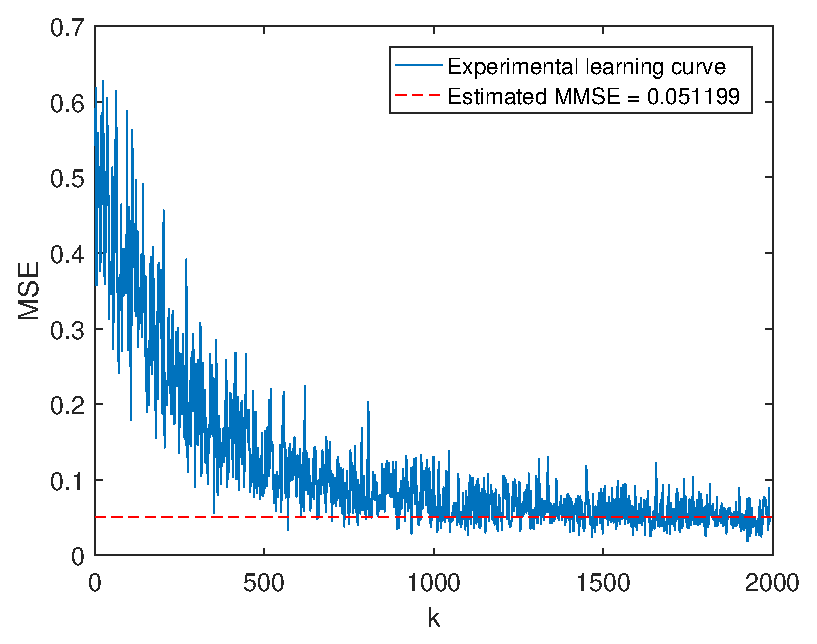
\includegraphics[scale=0.8]{part1_learning_curve.eps}
	\caption{Experimental learning curve for nonlinear plant indemnification using a linear filter. The learning curve was averaged 100 times.}
	\label{fig:part1-learning-curve}
\end{figure}
\FloatBarrier

\FloatBarrier
\begin{figure}[h!]
	\centering
	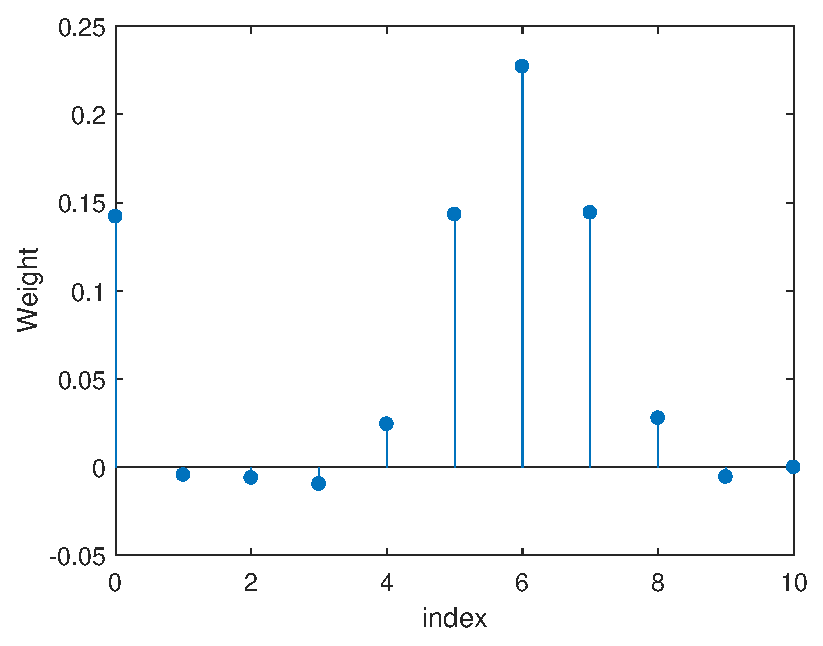
\includegraphics[scale=0.8]{part1_weights.eps}
	\caption{Weight vector after convergence.}
	\label{fig:part1-weights}
\end{figure}
\FloatBarrier

\subsubsection*{1.C}
As shown in Figure~\ref{fig:part1-learning-curve}, the MMSE estimated using the last 200 samples was equal to $\approx 0.051$.

\subsubsection*{1.D}
As discussed in class, the convergence time of the learning curve depends on the eigenvalues of the matrix $R$. Since $R$ is a diagonal matrix, its eigenvalues are equal to the entries in the main diagonal:
\begin{equation}
\lambda_1 = 1, \qquad \lambda_2 = \ldots = \lambda_{L+2} = \sigma_r^2.
\end{equation}

The time constants $\tau_n = 1/2\mu\lambda_n$ are therefore
\begin{equation}
\tau_1 = \frac{1}{2\mu}, \qquad \tau_2 = \ldots = \tau_{L+2} = \frac{1}{2\mu\sigma_r^2}.
\end{equation}

The learning curve has two modes. One due to the bias weight, and another due to the signal inputs. The slowest mode will determine the convergence time of the learning curve. 

In the first case, when $\sigma_r^2 = 4$, the slowest mode is due to the bias weight since $\tau_n < \tau_1, n > 1$. Therefore, the slowest time constant is $\tau_1 = 2050$. The approximate number of iterations for convergence is given by $(T_{mse})_1 = 0.5\tau_1 = 1025$, which we can verify this from Figure~\ref{fig:part1-learning-curve}.

When, $\sigma_r^2$ is made small. The mode due to the signal inputs will become the slowest one. And since we're assuming that $(L+1)\sigma_r^2 << 1$, the time constant due to the input signals is inversely proportional to the signal variance $\sigma_r^2$, as $\mu\approx 0.01$. Thus, the time constant is $\tau_n = 50/\sigma_r^2 >> 2050$. Therefore, the convergence time of the learning curve increases as we decrease the input signal power.

As for the MMSE, the MMSE is smaller for smaller $\sigma_r^2$. When the input signal is small enough to make the plant nonlinearity negligible, the plant is essentially the linear filter $\frac{1}{2}H_1(z)H_2(z)$, which is an FIR filter with 11 taps. The factor of $\frac{1}{2}$ appears because $g(x) \approx x/2, x \to 0$, which follows from the Taylor series expansion of $g(x)$. The adaptive filter has 10 taps plus the bias weight, and thus it could model the plant not perfectly, but very well. 

\subsubsection*{1.E}
The Matlab code is the same as for part (B) and it is shown below. The output of the plant is compared to the output of the adaptive filter in Figure~\ref{fig:part1-test}.

\FloatBarrier
\begin{figure}[h!]
	\centering
	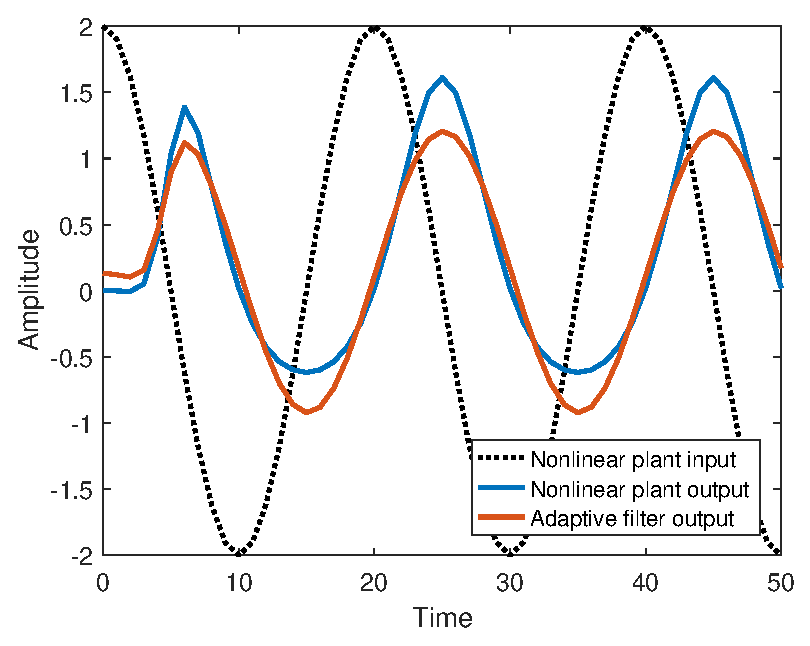
\includegraphics[scale=0.8]{part1_test.eps}
	\caption{Test of the adaptive filter after convergence with a sinusoidal signal. During the first $L+1$ samples, the filter was being initialized.}
	\label{fig:part1-test}
\end{figure}
\FloatBarrier

\singlespacing
\subsection*{Matalb code for part 1}
% This file was automatically created from the m-file 
% "m2tex.m" written by USL. 
% The fontencoding in this file is UTF-8. 
%  
% You will need to include the following two packages in 
% your LaTeX-Main-File. 
%  
% \usepackage{color} 
% \usepackage{fancyvrb} 
%  
% It is advised to use the following option for Inputenc 
% \usepackage[utf8]{inputenc} 
%  
  
% definition of matlab colors: 
\definecolor{mblue}{rgb}{0,0,1} 
\definecolor{mgreen}{rgb}{0.13333,0.5451,0.13333} 
\definecolor{mred}{rgb}{0.62745,0.12549,0.94118} 
\definecolor{mgrey}{rgb}{0.5,0.5,0.5} 
\definecolor{mdarkgrey}{rgb}{0.25,0.25,0.25} 
  
\DefineShortVerb[fontfamily=courier,fontseries=m]{\$} 
\DefineShortVerb[fontfamily=courier,fontseries=b]{\#} 
  
\noindent                                                                         
 \hspace*{-1.6em}{\scriptsize 1}$  $\color{mgrey}#%% Part 1: Modeling nonlinear plant with linear adaptive filter#\color{black}$$\\
 \hspace*{-1.6em}{\scriptsize 2}$  Niterations = 2000;             $\color{mgrey}$% Number of iterations$\color{black}$$\\
 \hspace*{-1.6em}{\scriptsize 3}$  Nruns = 100;                    $\color{mgrey}$% Number of runs to average MSE$\color{black}$$\\
 \hspace*{-1.6em}{\scriptsize 4}$  L = 9;                          $\color{mgrey}$% Memory length$\color{black}$$\\
 \hspace*{-1.6em}{\scriptsize 5}$  var_r = 4;                      $\color{mgrey}$% variance of input signal$\color{black}$$\\
 \hspace*{-1.6em}{\scriptsize 6}$  xtest = 2*cos(pi/10*(0:50));    $\color{mgrey}$% test signal$\color{black}$$\\
 \hspace*{-1.6em}{\scriptsize 7}$  ytest = nonlinear_plant(xtest); $\color{mgrey}$% nonlinear plant output for test signal$\color{black}$$\\
 \hspace*{-1.6em}{\scriptsize 8}$  Nweights = L + 2;               $\color{mgrey}$% number of weights: FIR taps + bias weight$\color{black}$$\\
 \hspace*{-1.6em}{\scriptsize 9}$  $\\
 \hspace*{-2em}{\scriptsize 10}$  $\color{mgrey}$% Calculate mu$\color{black}$$\\
 \hspace*{-2em}{\scriptsize 11}$  mu_max = 1/(var_r*(L+1) + 1);   $\color{mgrey}$% mu_max = 1/tr(R)$\color{black}$$\\
 \hspace*{-2em}{\scriptsize 12}$  mu = 0.01*mu_max;               $\color{mgrey}$% adaptation constant$\color{black}$$\\
 \hspace*{-2em}{\scriptsize 13}$  $\\
 \hspace*{-2em}{\scriptsize 14}$  $\color{mgrey}$% Adaptation using LMS$\color{black}$$\\
 \hspace*{-2em}{\scriptsize 15}$  MSE = zeros(Niterations, Nruns);$\\
 \hspace*{-2em}{\scriptsize 16}$  $#for#$ run = 1:Nruns$\\
 \hspace*{-2em}{\scriptsize 17}$      $\color{mgrey}$% Input signal: white and uniformly distributed zero-mean noise with$\color{black}$$\\
 \hspace*{-2em}{\scriptsize 18}$      $\color{mgrey}$% var_r variance$\color{black}$$\\
 \hspace*{-2em}{\scriptsize 19}$      r = sqrt(var_r*12)*(rand(Niterations, 1)-0.5);$\\
 \hspace*{-2em}{\scriptsize 20}$  $\\
 \hspace*{-2em}{\scriptsize 21}$      d = nonlinear_plant(r); $\color{mgrey}$% calculate desired response$\color{black}$$\\
 \hspace*{-2em}{\scriptsize 22}$      $\\
 \hspace*{-2em}{\scriptsize 23}$      $\color{mgrey}$% Reset weights, input, and error before running LMS$\color{black}$$\\
 \hspace*{-2em}{\scriptsize 24}$      W = zeros(Nweights, 1); $\color{mgrey}$% weight vector$\color{black}$$\\
 \hspace*{-2em}{\scriptsize 25}$      X = zeros(L+1, 1); $\color{mgrey}$% shift register$\color{black}$$\\
 \hspace*{-2em}{\scriptsize 26}$      error = zeros(Niterations, 1);$\\
 \hspace*{-2em}{\scriptsize 27}$      $#for#$ k = 1:Niterations$\\
 \hspace*{-2em}{\scriptsize 28}$          X = [r(k); X(1:end-1)];     $\color{mgrey}$% tap delay line$\color{black}$$\\
 \hspace*{-2em}{\scriptsize 29}$          Xin = [1; X];               $\color{mgrey}$% append input for bias weigth W(1)$\color{black}$$\\
 \hspace*{-2em}{\scriptsize 30}$          y = W.'*Xin;                $\color{mgrey}$% calculate output$\color{black}$$\\
 \hspace*{-2em}{\scriptsize 31}$          error(k) = d(k) - y;        $\color{mgrey}$% calculate error$\color{black}$$\\
 \hspace*{-2em}{\scriptsize 32}$          W = W + 2*mu*error(k)*Xin;  $\color{mgrey}$% weight update$\color{black}$$\\
 \hspace*{-2em}{\scriptsize 33}$      $#end#$$\\
 \hspace*{-2em}{\scriptsize 34}$      MSE(:, $\color{mdarkgrey}$run) = error.^2;$\color{black}$$\\
 \hspace*{-2em}{\scriptsize 35}$  $#end#$$\\
 \hspace*{-2em}{\scriptsize 36}$  $\\
 \hspace*{-2em}{\scriptsize 37}$  MSE = mean(MSE, 2); $\color{mgrey}$% average MSE over the number of runs$\color{black}$$\\
 \hspace*{-2em}{\scriptsize 38}$  MMSE = mean(MSE(end-199:end)); $\color{mgrey}$% use last 200 samples to estimate MMSE$\color{black}$$\\
 \hspace*{-2em}{\scriptsize 39}$  $\\
 \hspace*{-2em}{\scriptsize 40}$  $\color{mgrey}$% Ouput for test signal using linear model. W(1) is the bias weight$\color{black}$$\\
 \hspace*{-2em}{\scriptsize 41}$  ymodel = filter(W(2:end), 1, xtest) + W(1);$\\
 \hspace*{-2em}{\scriptsize 42}$  $\\
 \hspace*{-2em}{\scriptsize 43}$  $\color{mgrey}#%% Plots#\color{black}$$\\
 \hspace*{-2em}{\scriptsize 44}$  $\color{mgrey}$% Learning curve$\color{black}$$\\
 \hspace*{-2em}{\scriptsize 45}$  figure, $\color{mdarkgrey}$hold on, box on$\color{black}$$\\
 \hspace*{-2em}{\scriptsize 46}$  plot(MSE(L+1:end))$\\
 \hspace*{-2em}{\scriptsize 47}$  plot([1 Niterations], MMSE*[1 1], $\color{mdarkgrey}$'--r'$\color{black}$)$\\
 \hspace*{-2em}{\scriptsize 48}$  xlabel($\color{mdarkgrey}$'k'$\color{black}$, $\color{mdarkgrey}$'Fontsize'$\color{black}$, 12)$\\
 \hspace*{-2em}{\scriptsize 49}$  ylabel($\color{mdarkgrey}$'MSE'$\color{black}$, $\color{mdarkgrey}$'Fontsize'$\color{black}$, 12)$\\
 \hspace*{-2em}{\scriptsize 50}$  set(gca, $\color{mdarkgrey}$'Fontsize'$\color{black}$, 12)$\\
 \hspace*{-2em}{\scriptsize 51}$  legend($\color{mdarkgrey}$'Experimental learning curve'$\color{black}$, sprintf($\color{mdarkgrey}$'Estimated MMSE = %G'$\color{black}$, MMSE))$\\
 \hspace*{-2em}{\scriptsize 52}$  saveas(gca, $\color{mdarkgrey}$'figs/part1_learning_curve'$\color{black}$, $\color{mdarkgrey}$'epsc'$\color{black}$)$\\
 \hspace*{-2em}{\scriptsize 53}$  $\\
 \hspace*{-2em}{\scriptsize 54}$  $\color{mgrey}$% Weights$\color{black}$$\\
 \hspace*{-2em}{\scriptsize 55}$  figure, $\color{mdarkgrey}$hold on, box on$\color{black}$$\\
 \hspace*{-2em}{\scriptsize 56}$  stem(0:length(W)-1, W, $\color{mdarkgrey}$'fill'$\color{black}$)$\\
 \hspace*{-2em}{\scriptsize 57}$  xlabel($\color{mdarkgrey}$'index'$\color{black}$, $\color{mdarkgrey}$'Fontsize'$\color{black}$, 12)$\\
 \hspace*{-2em}{\scriptsize 58}$  ylabel($\color{mdarkgrey}$'Weight'$\color{black}$, $\color{mdarkgrey}$'Fontsize'$\color{black}$, 12)$\\
 \hspace*{-2em}{\scriptsize 59}$  set(gca, $\color{mdarkgrey}$'Fontsize'$\color{black}$, 12)$\\
 \hspace*{-2em}{\scriptsize 60}$  saveas(gca, $\color{mdarkgrey}$'figs/part1_weights'$\color{black}$, $\color{mdarkgrey}$'epsc'$\color{black}$)$\\
 \hspace*{-2em}{\scriptsize 61}$  $\\
 \hspace*{-2em}{\scriptsize 62}$  $\color{mgrey}$% Test signal$\color{black}$$\\
 \hspace*{-2em}{\scriptsize 63}$  figure, $\color{mdarkgrey}$hold on, box on$\color{black}$$\\
 \hspace*{-2em}{\scriptsize 64}$  t = 0:50;$\\
 \hspace*{-2em}{\scriptsize 65}$  plot(t, xtest, $\color{mdarkgrey}$':k'$\color{black}$, $\color{mdarkgrey}$'LineWidth'$\color{black}$, 2)$\\
 \hspace*{-2em}{\scriptsize 66}$  plot(t, ytest, $\color{mdarkgrey}$'LineWidth'$\color{black}$, 2)$\\
 \hspace*{-2em}{\scriptsize 67}$  plot(t, ymodel, $\color{mdarkgrey}$'LineWidth'$\color{black}$, 2)$\\
 \hspace*{-2em}{\scriptsize 68}$  xlabel($\color{mdarkgrey}$'Time'$\color{black}$, $\color{mdarkgrey}$'FontSize'$\color{black}$, 12)$\\
 \hspace*{-2em}{\scriptsize 69}$  ylabel($\color{mdarkgrey}$'Amplitude'$\color{black}$, $\color{mdarkgrey}$'FontSize'$\color{black}$, 12)$\\
 \hspace*{-2em}{\scriptsize 70}$  set(gca, $\color{mdarkgrey}$'Fontsize'$\color{black}$, 12)$\\
 \hspace*{-2em}{\scriptsize 71}$  legend($\color{mdarkgrey}$'Nonlinear plant input'$\color{black}$, $\color{mdarkgrey}$'Nonlinear plant output'$\color{black}$,...$\\
 \hspace*{-2em}{\scriptsize 72}$      $\color{mdarkgrey}$'Adaptive filter output'$\color{black}$, $\color{mdarkgrey}$'Location'$\color{black}$, $\color{mdarkgrey}$'SouthEast'$\color{black}$)$\\
 \hspace*{-2em}{\scriptsize 73}$  saveas(gca, $\color{mdarkgrey}$'figs/part1_test'$\color{black}$, $\color{mdarkgrey}$'epsc'$\color{black}$)$\\ 
  
\UndefineShortVerb{\$} 
\UndefineShortVerb{\#}
\doublespacing
%% Solutions to part 2
\pagebreak

\subsubsection*{2.A}


\subsubsection*{2.B}
The Matlab code to calculate the learning curve is included below. Figure~\ref{fig:part2-learning-curve} shows the learning curve averaged over 100 independent input realizations, and  Figure~\ref{fig:part2-weights} shows the converged weight vector. 

Note that the learning curve converged to a much smaller MMSE. Note further that the bias weight is practically negligible now, and some of the weights corresponding to the squared inputs and to the cross-products are significant. 

\FloatBarrier
\begin{figure}[h!]
	\centering
	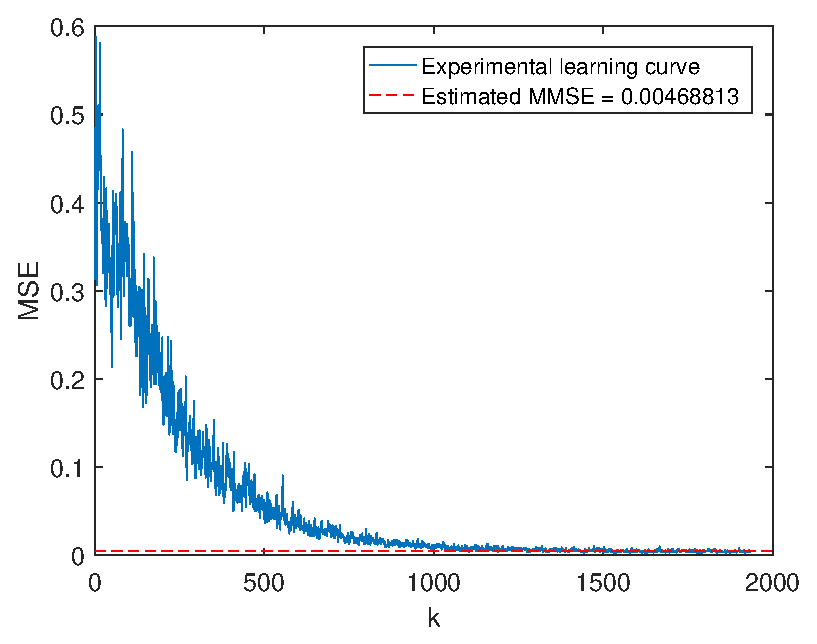
\includegraphics[scale=0.8]{part2_learning_curve.eps}
	\caption{Experimental learning curve for nonlinear plant identification using a nonlinear filter based on Volterra series. The learning curve was averaged 100 times. The training signal had variance $\sigma_r^2 = 4$.}
	\label{fig:part2-learning-curve}
\end{figure}
\FloatBarrier

\FloatBarrier
\begin{figure}[h!]
	\centering
	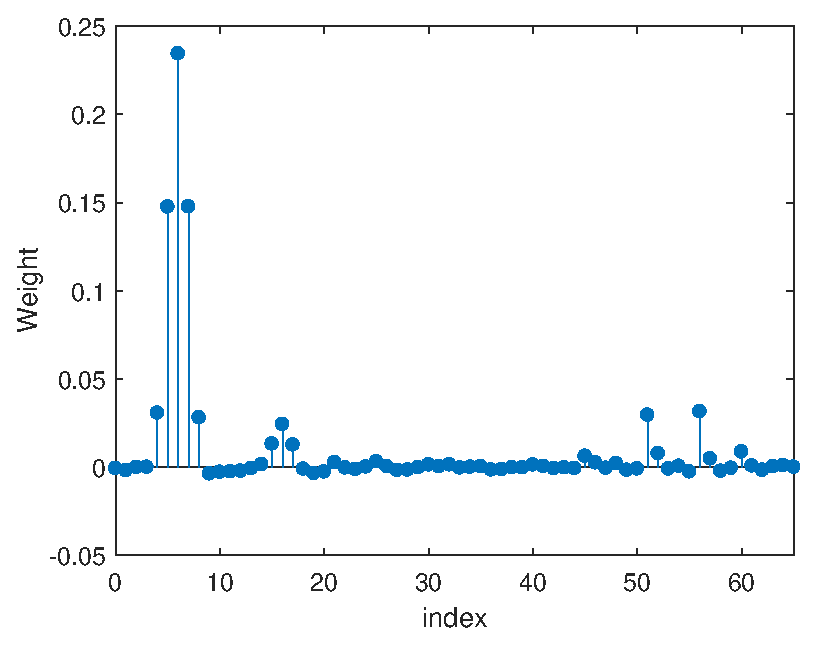
\includegraphics[scale=0.8]{part2_weights.eps}
	\caption{Weight vector after convergence.}
	\label{fig:part2-weights}
\end{figure}
\FloatBarrier

\subsubsection*{2.C}

As shown in Figure~\ref{fig:part2-learning-curve}, the MMSE estimated using the last 200 samples was equal to $\approx 0.0046$.

\subsubsection*{2.D}
The Matlab code is included in the appendix. The output of the plant is compared to the output of the adaptive filter in Figure~\ref{fig:part2-test}. 

The adaptive filter was trained with random signal, but it can almost perfectly track the plant output to a sinusoidal input. The same cannot be accomplished when the adaptive filter is linear as in part 1.E.

\FloatBarrier
\begin{figure}[h!]
	\centering
	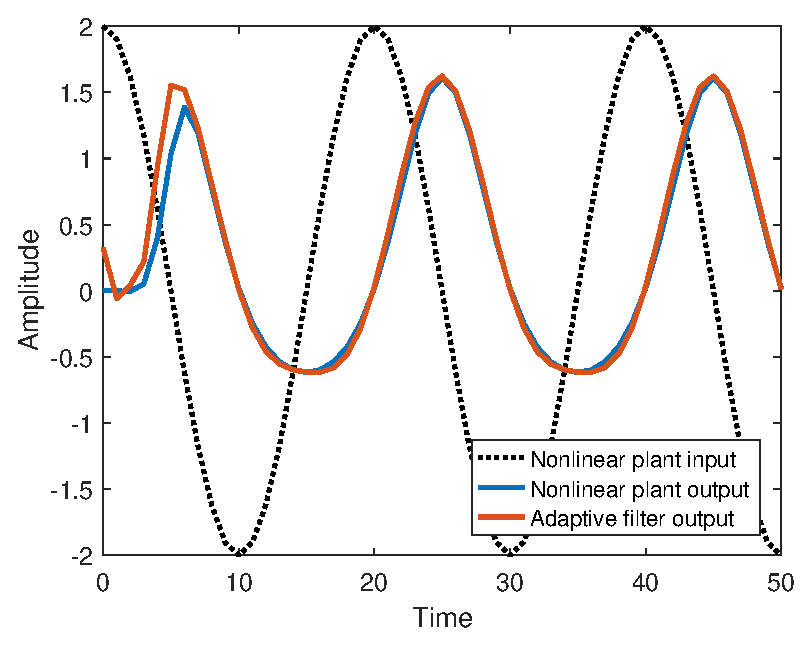
\includegraphics[scale=0.8]{part2_test.eps}
	\caption{Test of the adaptive filter after convergence with a sinusoidal signal. During the first $L+1$ samples, the filter was being initialized.}
	\label{fig:part2-test}
\end{figure}
\FloatBarrier

\subsubsection*{2.E}

When the training signal variance was $\sigma_r^2 = 0.4$, the adaptive filter achieved MMSE equal to $1.8\times 10^{-5}$ during training, but it didn't performed as well as before during test with a sinusoidal signal. The reason for this is that for a smaller training signals, the plant is approximately linear, and the adaptive equalizer cannot learn well the weights that weigh the nonlinear terms of the input. 

\FloatBarrier
\begin{figure}[h!]
	\centering
	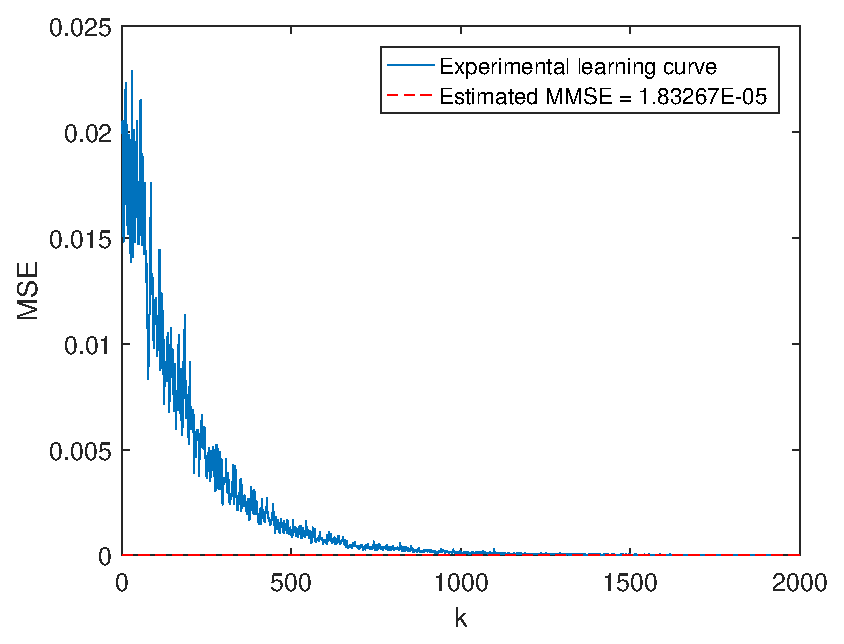
\includegraphics[scale=0.8]{part2e_learning_curve.eps}
	\caption{Experimental learning curve for nonlinear plant identification using a nonlinear filter based on Volterra series. The learning curve was averaged 100 times. The training signal had variance $\sigma_r^2 = 0.4$.}
	\label{fig:part2e-learning-curve}
\end{figure}
\FloatBarrier

\FloatBarrier
\begin{figure}[h!]
	\centering
	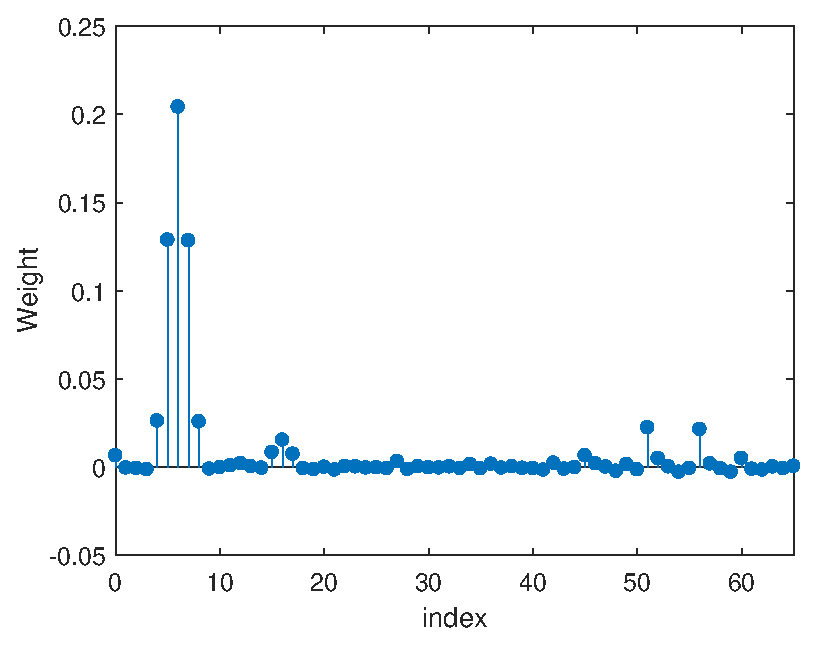
\includegraphics[scale=0.8]{part2e_weights.eps}
	\caption{Weight vector after convergence.}
	\label{fig:part2e-weights}
\end{figure}
\FloatBarrier

\FloatBarrier
\begin{figure}[t!]
	\centering
	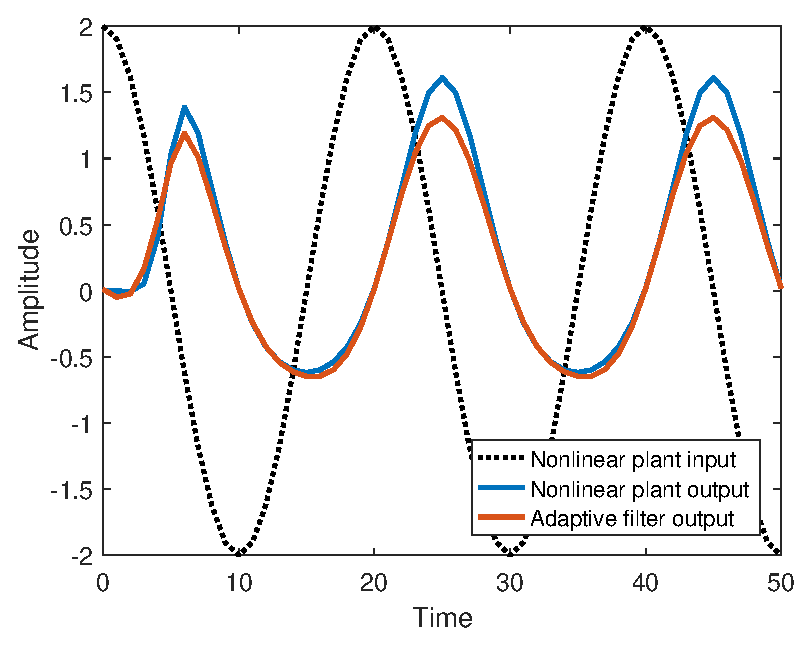
\includegraphics[scale=0.8]{part2e_test.eps}
	\caption{Test of the adaptive filter after convergence with a sinusoidal signal. During the first $L+1$ samples, the filter was being initialized.}
	\label{fig:part2e-test}
\end{figure}
\FloatBarrier

\singlespacing
\subsection*{Matalb code for part 2}
% This file was automatically created from the m-file 
% "m2tex.m" written by USL. 
% The fontencoding in this file is UTF-8. 
%  
% You will need to include the following two packages in 
% your LaTeX-Main-File. 
%  
% \usepackage{color} 
% \usepackage{fancyvrb} 
%  
% It is advised to use the following option for Inputenc 
% \usepackage[utf8]{inputenc} 
%  
  
% definition of matlab colors: 
\definecolor{mblue}{rgb}{0,0,1} 
\definecolor{mgreen}{rgb}{0.13333,0.5451,0.13333} 
\definecolor{mred}{rgb}{0.62745,0.12549,0.94118} 
\definecolor{mgrey}{rgb}{0.5,0.5,0.5} 
\definecolor{mdarkgrey}{rgb}{0.25,0.25,0.25} 
  
\DefineShortVerb[fontfamily=courier,fontseries=m]{\$} 
\DefineShortVerb[fontfamily=courier,fontseries=b]{\#} 
  
\noindent                                                                                      
 \hspace*{-1.6em}{\scriptsize 1}$  $\color{mgrey}#%% Part 2: Modeling nonlinear plant with nonlinear adaptive filter#\color{black}$$\\
 \hspace*{-1.6em}{\scriptsize 2}$  Niterations = 2000;             $\color{mgrey}$% Number of iterations$\color{black}$$\\
 \hspace*{-1.6em}{\scriptsize 3}$  Nruns = 100;                    $\color{mgrey}$% Number of runs to average MSE$\color{black}$$\\
 \hspace*{-1.6em}{\scriptsize 4}$  L = 9;                          $\color{mgrey}$% filter length - 1$\color{black}$$\\
 \hspace*{-1.6em}{\scriptsize 5}$  var_r = 4;                      $\color{mgrey}$% variance of input signal$\color{black}$$\\
 \hspace*{-1.6em}{\scriptsize 6}$  mu = 4e-4;                      $\color{mgrey}$% adaptation constant$\color{black}$$\\
 \hspace*{-1.6em}{\scriptsize 7}$  xtest = 2*cos(pi/10*(0:50));    $\color{mgrey}$% test signal$\color{black}$$\\
 \hspace*{-1.6em}{\scriptsize 8}$  ytest = nonlinear_plant(xtest); $\color{mgrey}$% nonlinear plant output for test signal$\color{black}$$\\
 \hspace*{-1.6em}{\scriptsize 9}$  Nweights = 2*(L+1) + nchoosek(L+1, 2) + 1; $\color{mgrey}$% Number of weights$\color{black}$$\\
 \hspace*{-2em}{\scriptsize 10}$  $\\
 \hspace*{-2em}{\scriptsize 11}$  $\color{mgrey}$% For part 2.E$\color{black}$$\\
 \hspace*{-2em}{\scriptsize 12}$  $\color{mgrey}$% var_r = 0.4;$\color{black}$$\\
 \hspace*{-2em}{\scriptsize 13}$  $\color{mgrey}$% mu = 4e-3;$\color{black}$$\\
 \hspace*{-2em}{\scriptsize 14}$  $\\
 \hspace*{-2em}{\scriptsize 15}$  $\color{mgrey}$% Indices for cross-products $\color{black}$$\\
 \hspace*{-2em}{\scriptsize 16}$  idx = nchoosek(1:L+1, 2);       $\\
 \hspace*{-2em}{\scriptsize 17}$  $\\
 \hspace*{-2em}{\scriptsize 18}$  MSE = zeros(Niterations, Nruns);$\\
 \hspace*{-2em}{\scriptsize 19}$  $#for#$ run = 1:Nruns$\\
 \hspace*{-2em}{\scriptsize 20}$      $\color{mgrey}$% Input signal: white and uniformly distributed zero-mean noise with$\color{black}$$\\
 \hspace*{-2em}{\scriptsize 21}$      $\color{mgrey}$% var_r variance$\color{black}$$\\
 \hspace*{-2em}{\scriptsize 22}$      r = sqrt(var_r*12)*(rand(Niterations, 1)-0.5); $\\
 \hspace*{-2em}{\scriptsize 23}$  $\\
 \hspace*{-2em}{\scriptsize 24}$      d = nonlinear_plant(r); $\color{mgrey}$% calculate desired response$\color{black}$$\\
 \hspace*{-2em}{\scriptsize 25}$      $\\
 \hspace*{-2em}{\scriptsize 26}$      $\color{mgrey}$% Reset weights, input, and error before running LMS$\color{black}$$\\
 \hspace*{-2em}{\scriptsize 27}$      W = zeros(Nweights, 1); $\color{mgrey}$% weight vector$\color{black}$$\\
 \hspace*{-2em}{\scriptsize 28}$      X = zeros(L+1, 1); $\color{mgrey}$% shift register$\color{black}$$\\
 \hspace*{-2em}{\scriptsize 29}$      error = zeros(Niterations, 1);$\\
 \hspace*{-2em}{\scriptsize 30}$      $#for#$ k = 1:Niterations$\\
 \hspace*{-2em}{\scriptsize 31}$          X = [r(k); X(1:end-1)];                 $\color{mgrey}$% tap delay line$\color{black}$$\\
 \hspace*{-2em}{\scriptsize 32}$          X2 = X.^2;                              $\color{mgrey}$% squared inputs $\color{black}$$\\
 \hspace*{-2em}{\scriptsize 33}$          Xprod  = X(idx(:, 1)).*X(idx(:, 2));    $\color{mgrey}$% cross-products$\color{black}$$\\
 \hspace*{-2em}{\scriptsize 34}$          Xin = [1; X; X2; Xprod];                $\color{mgrey}$% build input to adaptive filter$\color{black}$$\\
 \hspace*{-2em}{\scriptsize 35}$          y = W.'*Xin;                            $\color{mgrey}$% calculate output$\color{black}$$\\
 \hspace*{-2em}{\scriptsize 36}$          error(k) = d(k) - y;                    $\color{mgrey}$% calculate error$\color{black}$$\\
 \hspace*{-2em}{\scriptsize 37}$          W = W + 2*mu*error(k)*Xin;              $\color{mgrey}$% weights update$\color{black}$$\\
 \hspace*{-2em}{\scriptsize 38}$      $#end#$$\\
 \hspace*{-2em}{\scriptsize 39}$      MSE(:, $\color{mdarkgrey}$run) = error.^2;$\color{black}$$\\
 \hspace*{-2em}{\scriptsize 40}$  $#end#$$\\
 \hspace*{-2em}{\scriptsize 41}$  $\\
 \hspace*{-2em}{\scriptsize 42}$  MSE = mean(MSE, 2); $\color{mgrey}$% average MSE over the number of runs$\color{black}$$\\
 \hspace*{-2em}{\scriptsize 43}$  MMSE = mean(MSE(end-199:end)); $\color{mgrey}$% use last 200 samples to estimate MMSE$\color{black}$$\\
 \hspace*{-2em}{\scriptsize 44}$  $\\
 \hspace*{-2em}{\scriptsize 45}$  $\color{mgrey}$% Calculate model output for test signal$\color{black}$$\\
 \hspace*{-2em}{\scriptsize 46}$  ymodel = zeros(size(xtest));$\\
 \hspace*{-2em}{\scriptsize 47}$  $#for#$ k = 1:length(xtest)$\\
 \hspace*{-2em}{\scriptsize 48}$      X = [xtest(k); X(1:end-1)];$\\
 \hspace*{-2em}{\scriptsize 49}$      X2 = X.^2;$\\
 \hspace*{-2em}{\scriptsize 50}$      Xprod  = X(idx(:, 1)).*X(idx(:, 2));$\\
 \hspace*{-2em}{\scriptsize 51}$      Xin = [1; X; X2; Xprod];$\\
 \hspace*{-2em}{\scriptsize 52}$      ymodel(k) = W.'*Xin;$\\
 \hspace*{-2em}{\scriptsize 53}$  $#end#$$\\
 \hspace*{-2em}{\scriptsize 54}$  $\\
 \hspace*{-2em}{\scriptsize 55}$  $\color{mgrey}#%% Plots#\color{black}$$\\
 \hspace*{-2em}{\scriptsize 56}$  $\color{mgrey}$% Learning curve$\color{black}$$\\
 \hspace*{-2em}{\scriptsize 57}$  figure, $\color{mdarkgrey}$hold on, box on$\color{black}$$\\
 \hspace*{-2em}{\scriptsize 58}$  plot(MSE(Nweights+1:end, $\color{mdarkgrey}$:))$\color{black}$$\\
 \hspace*{-2em}{\scriptsize 59}$  plot([1 Niterations], MMSE*[1 1], $\color{mdarkgrey}$'--r'$\color{black}$)$\\
 \hspace*{-2em}{\scriptsize 60}$  xlabel($\color{mdarkgrey}$'k'$\color{black}$, $\color{mdarkgrey}$'Fontsize'$\color{black}$, 12)$\\
 \hspace*{-2em}{\scriptsize 61}$  ylabel($\color{mdarkgrey}$'MSE'$\color{black}$, $\color{mdarkgrey}$'Fontsize'$\color{black}$, 12)$\\
 \hspace*{-2em}{\scriptsize 62}$  set(gca, $\color{mdarkgrey}$'Fontsize'$\color{black}$, 12)$\\
 \hspace*{-2em}{\scriptsize 63}$  legend($\color{mdarkgrey}$'Experimental learning curve'$\color{black}$, sprintf($\color{mdarkgrey}$'Estimated MMSE = %G'$\color{black}$, MMSE))$\\
 \hspace*{-2em}{\scriptsize 64}$  saveas(gca, $\color{mdarkgrey}$'figs/part2_learning_curve'$\color{black}$, $\color{mdarkgrey}$'epsc'$\color{black}$)$\\
 \hspace*{-2em}{\scriptsize 65}$  $\\
 \hspace*{-2em}{\scriptsize 66}$  $\color{mgrey}$% Weights$\color{black}$$\\
 \hspace*{-2em}{\scriptsize 67}$  figure, $\color{mdarkgrey}$hold on, box on$\color{black}$$\\
 \hspace*{-2em}{\scriptsize 68}$  stem(0:Nweights-1, W, $\color{mdarkgrey}$'fill'$\color{black}$)$\\
 \hspace*{-2em}{\scriptsize 69}$  xlabel($\color{mdarkgrey}$'index'$\color{black}$, $\color{mdarkgrey}$'Fontsize'$\color{black}$, 12)$\\
 \hspace*{-2em}{\scriptsize 70}$  ylabel($\color{mdarkgrey}$'Weight'$\color{black}$, $\color{mdarkgrey}$'Fontsize'$\color{black}$, 12)$\\
 \hspace*{-2em}{\scriptsize 71}$  set(gca, $\color{mdarkgrey}$'Fontsize'$\color{black}$, 12)$\\
 \hspace*{-2em}{\scriptsize 72}$  axis([0 $\color{mdarkgrey}$Nweights-1 -0.05 0.25])$\color{black}$$\\
 \hspace*{-2em}{\scriptsize 73}$  saveas(gca, $\color{mdarkgrey}$'figs/part2_weights'$\color{black}$, $\color{mdarkgrey}$'epsc'$\color{black}$)$\\
 \hspace*{-2em}{\scriptsize 74}$  $\\
 \hspace*{-2em}{\scriptsize 75}$  $\color{mgrey}$% Test signal$\color{black}$$\\
 \hspace*{-2em}{\scriptsize 76}$  figure, $\color{mdarkgrey}$hold on, box on$\color{black}$$\\
 \hspace*{-2em}{\scriptsize 77}$  t = 0:50;$\\
 \hspace*{-2em}{\scriptsize 78}$  plot(t, xtest, $\color{mdarkgrey}$':k'$\color{black}$, $\color{mdarkgrey}$'LineWidth'$\color{black}$, 2)$\\
 \hspace*{-2em}{\scriptsize 79}$  plot(t, ytest, $\color{mdarkgrey}$'LineWidth'$\color{black}$, 2)$\\
 \hspace*{-2em}{\scriptsize 80}$  plot(t, ymodel, $\color{mdarkgrey}$'LineWidth'$\color{black}$, 2)$\\
 \hspace*{-2em}{\scriptsize 81}$  xlabel($\color{mdarkgrey}$'Time'$\color{black}$, $\color{mdarkgrey}$'FontSize'$\color{black}$, 12)$\\
 \hspace*{-2em}{\scriptsize 82}$  ylabel($\color{mdarkgrey}$'Amplitude'$\color{black}$, $\color{mdarkgrey}$'FontSize'$\color{black}$, 12)$\\
 \hspace*{-2em}{\scriptsize 83}$  legend($\color{mdarkgrey}$'Nonlinear plant input'$\color{black}$, $\color{mdarkgrey}$'Nonlinear plant output'$\color{black}$,...$\\
 \hspace*{-2em}{\scriptsize 84}$      $\color{mdarkgrey}$'Adaptive filter output'$\color{black}$, $\color{mdarkgrey}$'Location'$\color{black}$, $\color{mdarkgrey}$'SouthEast'$\color{black}$)$\\
 \hspace*{-2em}{\scriptsize 85}$  set(gca, $\color{mdarkgrey}$'Fontsize'$\color{black}$, 12)$\\
 \hspace*{-2em}{\scriptsize 86}$  saveas(gca, $\color{mdarkgrey}$'figs/part2_test'$\color{black}$, $\color{mdarkgrey}$'epsc'$\color{black}$)$\\ 
  
\UndefineShortVerb{\$} 
\UndefineShortVerb{\#}

\end{document}
